% \iffalse
\let\negmedspace\undefined
\let\negthickspace\undefined
\documentclass[journal,12pt,twocolumn]{IEEEtran}
\usepackage{cite}
\usepackage{amsmath,amssymb,amsfonts,amsthm}
\usepackage{algorithmic}
\usepackage{graphicx}
\usepackage{textcomp}
\usepackage{xcolor}
\usepackage{txfonts}
\usepackage{listings}
\usepackage{enumitem}
\usepackage{mathtools}
\usepackage{gensymb}
\usepackage{comment}
\usepackage[breaklinks=true]{hyperref}
\usepackage{tkz-euclide} 
\usepackage{listings}
\usepackage{gvv}                                        
\def\inputGnumericTable{}                                 
\usepackage[latin1]{inputenc}                                
\usepackage{color}                                            
\usepackage{array}                                            
\usepackage{longtable}                                       
\usepackage{calc}                                             
\usepackage{multirow}                                         
\usepackage{hhline}                                           
\usepackage{ifthen}                                           
\usepackage{lscape}
\usepackage{placeins}
\usepackage{xparse}


\newtheorem{theorem}{Theorem}[section]
\newtheorem{problem}{Problem}
\newtheorem{proposition}{Proposition}[section]
\newtheorem{lemma}{Lemma}[section]
\newtheorem{corollary}[theorem]{Corollary}
\newtheorem{example}{Example}[section]
\newtheorem{definition}[problem]{Definition}
\newcommand{\BEQA}{\begin{eqnarray}}
\newcommand{\EEQA}{\end{eqnarray}}
\newcommand{\define}{\stackrel{\triangle}{=}}
\theoremstyle{remark}
\newtheorem{rem}{Remark}

\graphicspath{ {./figs/} } 

\begin{document}

\bibliographystyle{IEEEtran}
\vspace{3cm}

\Large\title{NCERT Question 10.5.2.5}
\large\author{EE23BTECH11032 - Kaustubh Parag Khachane $^{*}$% <-this % stops a space
}
\maketitle
\newpage
\bigskip

\renewcommand{\thefigure}{\theenumi}
\renewcommand{\thetable}{\theenumi}
\large\textbf{Question 10.5.2.5} : \normalsize Find the number of terms in each of the following APs. Then express each term as x(n) and find the z transform and its ROC: 

\brak{i} 7, 13, 19, ... 205

\brak{ii} 18, 15$\frac{1}{2}$, 13, ... -47


\large\textbf{Solution} :\normalsize

\begin{table}[!ht] 
\centering
\setlength{\extrarowheight}{8pt}
\begin{tabular}{|l|l|l|}
    \hline
    \textbf{Parameter} & \textbf{Description} & \textbf{Value} \\
    \hline
     m & Mass of object & 10 Kg \\\hline
     $\mu$ & Frictional coefficient \brak{static} & 0.25\\\hline
     x\brak{t} & Displacement of block &  \\\hline
     $x\brak{0}$ & Initial displacement & 0 \brak{assumed} \\\hline
     g & Gravitational acceleration & 10 $m/s^2$ \\\hline
     $F_s$ & Spring force &  \\\hline
     f & frictional force &  $\mu$ N \\\hline
     N & Normal Force & mg $cos\brak{\theta}$ \\\hline
    \end{tabular}
  \vspace{4mm}
 \caption{Parameter Table}
 \label{tab:table0_xe80}
\end{table}

The number of terms in the AP x(n) is given by : 
\begin{align}  \label{eq:eq12}
    \frac{x\brak{n} - x\brak{0}}{d} + 1
\end{align}
\textbf{\brak i} 

$x_{1}\brak{n} = 205$\\ 
Using \eqref{eq:eq12}, Number of terms in the AP is : 
\begin{align}
\frac{205 - 7}{6} + 1 = 34\\
\end{align}
$\therefore$ There are 34 elements in the series.

\textbf{\brak{ii}} 

$x_{2}\brak{n} = -47$\\ 
Using \eqref{eq:eq12}, Number of terms in the AP is :
\begin{align}
\frac{-47 - 18}{-2\frac{1}{2}} + 1 = 27
\end{align}
$\therefore$ There are 27 elements in the series.

Finding the z transform and ROC : \\
\begin{align}
\text{For an AP } x\brak{n} &= \sbrak{x\brak{0} + nd}u\brak{n}\\
&=x\brak{0}u\brak{n} + dnu\brak{n}\label{eq:eq2}
\end{align}
\begin{align}
   z\{u\brak{n}\} &=  U\brak{z} = \frac{1}{1 - z^{-1}} , |z| > 1\label{eq:eq4}\\
   z\{nu\brak{n}\} &= -z\frac{dU\brak{z}}{dz} = \frac{z^{-1}}{\brak{1-z^{-1}}^2},|z| > 1 \label{eq:eq5}
\end{align}
ROC is given by values of z for which :
\begin{align}
    \lvert X\brak{z}\rvert = \sum_{n = -\infty}^{\infty}\lvert x\brak{n}z^{-n}\rvert < \infty
\end{align}
Using equations \eqref{eq:eq4} and \eqref{eq:eq5} in equation \eqref{eq:eq2} :
\begin{align}\label{eq:eq3}
    z\{x\brak{n}\} = X(z) = \frac{x\brak{0}}{1 - z^{-1}} + d\frac{z^{-1}}{\brak{1-z^{-1}}^2}
\end{align}
\textbf{\brak{i}}

$x_{1}\brak{n} = \brak{7 + \brak{n}6}u\brak{n}$
\begin{align}
     x_{1}\brak{n} & = \begin{cases} 
        0 & \text{for } n < 0 \\
        7 + \brak{n}6 & \text{for } n \geq 0
    \end{cases}
\end{align}
Using the values in \tabref{table0} and equation \eqref{eq:eq3} :
\begin{align}
X_{1}\brak{z} &= \frac{7}{1 - z^{-1}} + \frac{6z^{-1}}{\brak{1 - z^{-1}}^2}\\
 &= \frac{7 - z^{-1}}{\brak{1-z^{-1}}^2}
 \end{align}
 The ROC is $|z|>1$ as it is an AP.
 
\textbf{\brak{ii}}

$x_{2}\brak{n} = \brak{18 + n\brak{-2\frac{1}{2}}}u\brak{n}$\\
\begin{align}
     x_{2}\brak{n} & = \begin{cases}
        0 & \text{for } n < 0 \\
        18 + n\brak{-2\frac{1}{2}} & \text{for } n \geq 0
    \end{cases}
 \end{align}
Using the values in \tabref{table0} and equation \eqref{eq:eq3} :
\begin{align} 
X_{2}\brak{z} &=  \frac{18}{1 - z^{-1}} - \brak{2\frac{1}{2}}\frac{z^{-1}}{\brak{1-z^{-1}}^2}\\
&= \frac{18 - \brak{20\frac{1}{2}}z^{-1}}{\brak{1 - z^{-1}}^2}
\end{align}

The ROC is $|z|>1$ as it is an AP.

\newpage
The graphs for x\brak{n} : \\
\large\textbf{\brak{i}} \normalsize The graph of $x_{1}$\brak{n} is :
\begin{figure}[ht]
    \begin{center}
    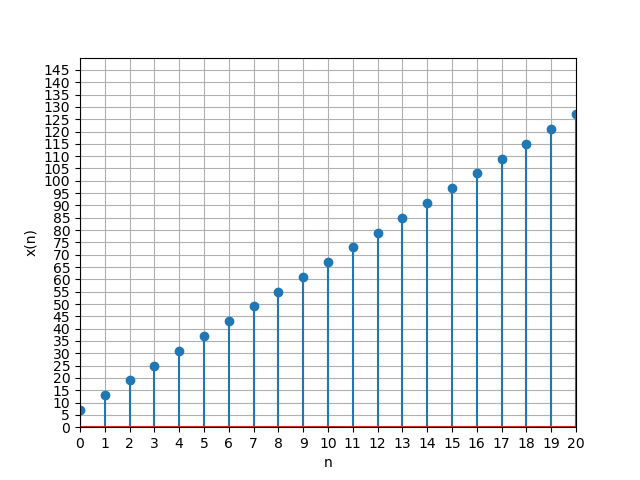
\includegraphics[width = 8cm]{Figure_1}\\
    Fig. 0. Plot of x\brak{n} \\
    \end{center}
\end{figure}

\large\textbf{\brak{ii}} \normalsize The graph of $x_{2}$\brak{n} is :
\begin{figure}[!ht]
    \begin{center}
    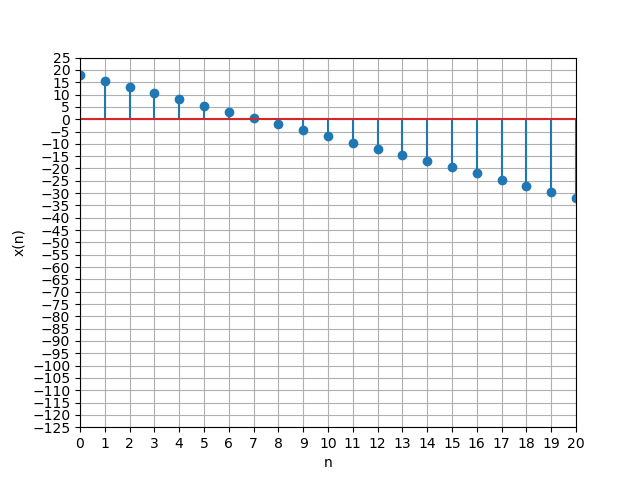
\includegraphics[width = 8cm]{Figure_2}\\
    Fig. 1. Plot of x\brak{n} \\
    \end{center}
\end{figure}

\end{document}
